\documentclass{article}

% load tikz core package
\usepackage{tikz}

% load aditional tikz packages
\usetikzlibrary{
  arrows.meta,
  decorations.pathmorphing,
  backgrounds,
  positioning,
  fit,
  petri
}

% tikz options
\tikzset{
  node distance=1.3cm,
  bend angle=45,
  auto,
  on grid,
  >={Stealth[round]},
  % styles
  blue/.style={
    draw=blue!75,
    fill=blue!20,
  },
  every place/.style={
    blue,  
    minimum size=6mm,
    thick,
  },
  every transition/.style={
    blue,
    thick,
  },
  every label/.style={red},
  red place/.style={
    place,
    draw=red!75,
    fill=red!20,
  }
} 

\begin{document}
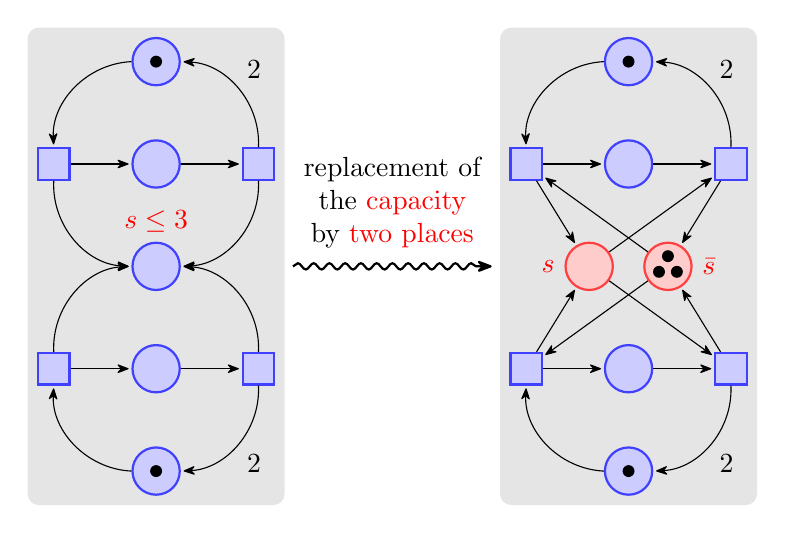
\begin{tikzpicture}
  % places
  \node [place, tokens=1] (w1)                                   {};
  \node [place]           (c1) [below=of w1]                     {};
  \node [place]           (s)  [below=of c1,label=above:$s\leq3$]{};
  \node [place]           (c2) [below=of s]                      {};
  \node [place, tokens=1] (w2) [below=of c2]                     {};

  % transitions
  \node [transition] (e1) [left=of c1] {}
  edge [pre,bend left] (w1)
  edge [post,bend right] (s)
  edge [post] (c1);
  \node [transition] (e2) [left=of c2] {}
  edge [pre,bend right] (w2)
  edge [post,bend left] (s)
  edge [post] (c2);
  \node [transition] (l1) [right=of c1] {}
  edge [pre] (c1)
  edge [post,bend left] (s)
  edge [post, bend right] node[swap] {2} (w1);
  \node [transition] (l2) [right=of c2] {}
  edge [pre] (c2)
  edge [post,bend right] (s)
  edge [post,bend left] node {2} (w2);

  \begin{scope}[xshift=6cm]
    \node [place,tokens=1]     (w1')                            {};
    \node [place]              (c1') [below=of w1']             {};
    \node [red place]          (s1') [below=of c1',xshift=-5mm]
    [label=left:$s$]                                    {};
    \node [red place,tokens=3] (s2') [below=of c1',xshift=5mm]
    [label=right:$\bar s$]                              {};
    \node [place]              (c2') [below=of s1',xshift=5mm]  {};
    \node [place,tokens=1]     (w2') [below=of c2']             {};

    \node [transition] (e1') [left=of c1'] {}
    edge [pre,bend left]                  (w1')
    edge [post]                           (s1')
    edge [pre]                            (s2')
    edge [post]                           (c1');
    \node [transition] (e2') [left=of c2'] {}
    edge [pre,bend right]                 (w2')
    edge [post]                           (s1')
    edge [pre]                            (s2')
    edge [post]                           (c2');
    \node [transition] (l1') [right=of c1'] {}
    edge [pre]                            (c1')
    edge [pre]                            (s1')
    edge [post]                           (s2')
    edge [post,bend right] node[swap] {2} (w1');
    \node [transition] (l2') [right=of c2'] {}
    edge [pre]                            (c2')
    edge [pre]                            (s1')
    edge [post]                           (s2')
    edge [post,bend left]  node {2}       (w2');
  \end{scope}

  \begin{scope}[on background layer]
    \node (r1) [fill=black!10,rounded corners,fit=(w1)(w2)(e1)(e2)(l1)(l2)] {};
    \node (r2) [fill=black!10,rounded corners,fit=(w1')(w2')(e1')(e2')(l1')(l2')] {};
  \end{scope}

  \draw [shorten >=1mm,->,thick,decorate,
         decoration={snake,amplitude=.4mm,segment length=2mm,
                     pre=moveto,pre length=1mm,post length=2mm}]
    (r1) -- (r2) node [above=1mm,midway,text width=3cm,align=center]
      {replacement of the \textcolor{red}{capacity} by \textcolor{red}{two places}};
\end{tikzpicture}
\end{document}